\chapter{Experimental protocol}
\label{Chap3}

In this part I will focus on the relevant tests made, results of the first tests will be found in Appendix \ref{badtests}.

    \section{Parameters}
    
        The following table describes the different devices used for the realization of the samples and shows the parameters that have to be taken into account during the fabrication. The parameters in bold are the most influent in the results we will obtain, so they are important and the settings needs to be determined precisely.
        
       \vspace{0.5cm}
         
        \begin{tabular}{|c|c|c|}
        \hline
        \textsc{Step}&\textsc{Device}&\textsc{Parameters}\\
        \hline
        Resist deposition&Spinner&Rotation Speed\\
        \hline
        Resist baking&Hot plate&Temperature\\
        \hline
        Pattern design&EBL&\textbf{Dose}, \textbf{Shape(area)}, Resolution\\
        \hline
        Development&MIBK, MG, IPA&\textbf{Duration}\\ 
        \hline
        Deposition of metal&Evaporator&\textbf{Angle}\\
        \hline
        Oxidation&Evaporator&\textbf{Pressure}, \textbf{Duration}\\
        \hline
        Plasma Etching&Plasma gun&\textbf{Duration}, Position\\
        \hline
        Lift-off&Aceton&$\varnothing$ \\
        \hline
        \end{tabular}
        
        \vspace{0.5cm}
        
            
            The chip we realize consists in twenty samples, with four different surface areas (0.5, 1, 1.5 \& 2 $\mu m^2$) and five different electron doses (from 2000 to 3000 by 250 $c/\mu m^2$) in the EBL. This gives us some statistics : we do not stick to one result but we have several ones to make sure the datas we get are relevant and not due to any problem. Moreover, some little troubles can always occur on one of the samples (EBL default, speck of dust...) and fabricating 20 of them avoids to loose a whole attempt. Mathieu already defined some settings such as the development time and he made the patterns and the EBL writing.
                        
        \section{Experimental procedure}
        
            In order to have coherent results I have always followed the same process to realize the samples. Based on 4 layers of MMA and one layer of PMMA and EBL dose from 2000 to 3000 $\mu m^2$, according to the pattern in Fig. \ref{patternjunction}, I develop 20s in MIBK, 20s in MG and IPA. Then I evaporate 20nm of Al. Depending on the sample I want to make, I can strongly oxidize with a pressure of 200mbar of O$_2$ during 10 min. Then, I can use the plasma to etch, the parameters are a pressure of $4.10^{-4}mbar$ of Argon, a power of 40mA, an extraction voltage of -0.8kV (lowered down to -250V in July, due to problems that high voltage caused) and a Ion Energy of 1.5kV. I can also oxidize with a pressure of 2mbar during 2min. Finally, I evaporate 25nm of Cu before letting the sample in lift-off for more than an hour..
            
            I have realized samples with strong oxidation and plasma etching to see how much oxide was etched, then I have realized samples with strong oxidation, plasma etching and regular oxidation and regular oxidation reference samples in order to cool them down to see the differences and so the effect of the plasma on the quality of the NIS junction.  You can find an exhaustive table of the parameters used for each test in Appendix \ref{parametertable}
            
            \begin{figure}
                \centering
                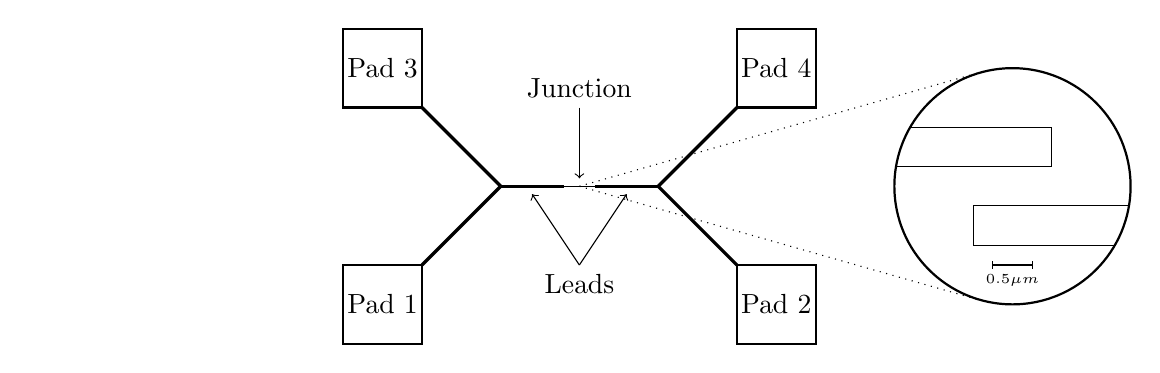
\begin{tikzpicture}
                    \draw [thick](0,0)--++(1,0)--++(0,1)--++(-1,0)--cycle;
                    \draw [thick](0,3)--++(1,0)--++(0,1)--++(-1,0)--cycle;
                    \draw [thick](5,0)--++(1,0)--++(0,1)--++(-1,0)--cycle;
                    \draw [thick](5,3)--++(1,0)--++(0,1)--++(-1,0)--cycle;
                    \draw [very thick](1,1)--(2,2);
                    \draw [very thick](1,3)--(2,2);
                    \draw [very thick](5,1)--(4,2);
                    \draw [very thick](5,3)--(4,2);
                    \draw [very thick](2,2)--(2.8,2);
                    \draw [very thick](4,2)--(3.2,2);
                    \draw (2.8,2)--(3.2,2);
                    \draw [->] (3,3)--(3,2.1);
                    \draw (3,3)node[above]{Junction};
                    \draw (0.5,0.5)node{Pad 1};
                    \draw (0.5,3.5) node{Pad 3};
                    \draw (5.5,0.5)node{Pad 2};
                    \draw (5.5,3.5)node{Pad 4};
                    \draw [->] (3,1)--(2.4,1.9);
                    \draw [->] (3,1)--(3.6,1.9);
                    \draw (3,1)node[below]{Leads};
                    \draw [dotted,thin] (3,2)--(8.1,3.45);
                    \draw [dotted,thin] (3,2)--(8.1,0.55);
                    \draw [thick](8.5,2) circle(1.5);
                    \draw (7.2,2.75)--(9,2.75)--(9,2.25)--(7.02,2.25);
                    \draw (9.8,1.25)--(8,1.25)--(8,1.75)--(9.98,1.75);
                    \draw (8.25,1.05)--(8.25,0.95);
                    \draw (8.75,1.05)--(8.75,0.95);
                    \draw (8.25,1)--(8.75,1)node[midway, below]{\tiny{0.5$\mu m$}};
                    \draw [color=white](-4,2)--(-4,2.01);
                \end{tikzpicture}
                \caption{Pattern of the junctions}
                \label{patternjunction}
            \end{figure}
            
            \section{Problems with the devices}
            
            When I was here, there have been some problems with the evaporator LISA which I used to make the structures. The plasma gun seemed to have a problem in the begining of July, since it didn't work properly. We could see that nothing happened when we set the power current. It was cleaned and repaired and the main user advised to limit the Extraction to -250V to avoid future breakdown. After this, the plasma seemed to act differently, it seemed more powerful according to the results (See \ref{Chap4}). Then, just before I left, everyone seemed to have troubles with the junctions made in the evaporator. I tried to 
            
            \section{Measurement setup}
            \subsection{Room temperature setup}
            
            We first used a method to measure the samples but it was not rigorous enough, I talk about it in Appendix \ref{badmeasures}.
                
                Let's focus on the good measurements. I have made four-probe resistance measurements on the samples I have fabricated with a probe station. The four-probe measurements make sense as it is the only way to measure the real resistance of the device, without parasite resistances. The probestation make a slope of voltage from -100 mV to 100 mV, measure the voltage and the current between two electrodes and trace an I-V curve. It export the data obtained in .DAT files with the current and voltage tables. I have then realized a Matlab program to exploit them efficiently and be able to trace charts showing the more parameter dependances possible.
                
            \subsection{Low temperature setup}
                
                Since the samples I make are superconductors-based structures, it is worth measuring them at low temperature to have the superconductivity state of Al. The critical temperature of Al is 1.2K, so we have to cool the sample lower than this temperature to obtain results. We use a dilution cryostat as the ones described earlier. Once the sample is cold, we can start the measurements.
                
                There are devices that can be connected to the cryostat lines wich are lined to the samples. Everything is controlled through Matlab programs. I have adapted an existing program to make it fit better with the measurements I wanted to do and the way I wanted to exploit the datas. First, I have to set the parameters, then the program is linked with the devices, it controls the generator to make a voltage slope and in the meanwhile it asks the multiplexer to get the bias voltage and the voltage which comes from the current amplifier (See Fig.\ref{circuit}). These are rough values that are not the real ones. I can draw IV curves to check that everything is correct : good $V_bias$ range, accurate current amplification... Then the program saves the datas that I will exploit with a better program later. The program I wrote allows to draw the IV curves, and determine easily the resistance and the leakage of the junctions.
                                
        \begin{figure}
            \centering
            \begin{circuitikz}
                \draw 
            (0,0) node[ground]{} 
                to [V,v=$DC$,v_>=$V_{meas}$] (0,3)
                to [R=5<\kilo\ohm>] (3,3)
                to [R=20<\ohm>,*-,v_<=$V_{bias}$] (3,0)
                node[ground] {}
            (3,3) to [R=$R_{sample}$,i=$i_{sample}$] (8,3)
                to [ammeter, v^<=$V->I_{amplifed}$] (8,0) node[ground] {}
            ;
            \end{circuitikz}
            \caption{Schematics of the set up for low temperature measurements}
         \label{circuit}
        \end{figure}
        
                
                
                
                
                
                
            
